% ============================================================================
% moe_bias_report_acm_v2.tex
% ACM sigconf draft -- honest re-analysis of expt-bias-1 (routing-Shapley
% attribution of social bias over MoE experts).
% Compile (self-contained, thebibliography embedded): pdflatex file.tex
% Figures: stats_analysis/figures/ (path set via \graphicspath below).
%
% Ladder point estimates and subset verdicts were read from
% stats_analysis/outputs/s03_h1_verdict.json (v1 ladder rows, exact
% two-sided permutation p); 95%% block-bootstrap CIs from
% stats_analysis/outputs/s04_bootstrap_cis.json; dense baselines from
% results/*/result.json ("concentration_metrics"). Rows/entries whose
% measurements remain flight-flagged are marked in Section~\ref{sec:limits}
% and with footnote markers in the tables.
% ============================================================================
\documentclass[sigconf]{acmart}
\settopmatter{printacmref=false}
\renewcommand\footnotetextcopyrightpermission[1]{}
\setcopyright{none}
\setcitestyle{numbers}
\setlength{\emergencystretch}{3em}
\setlength{\headheight}{15.3pt}

\begin{CCSXML}
<ccs2012>
<concept>
<concept_id>10010147.10010178</concept_id>
<concept_desc>Computing methodologies~Artificial intelligence</concept_desc>
<concept_significance>300</concept_significance>
</concept>
</ccs2012>
\end{CCSXML}
\ccsdesc[300]{Computing methodologies~Artificial intelligence}

\begin{document}

\title{Does Expert Sparsity Concentrate Social Bias?\\
  A Routing-Shapley Re-Analysis of Mixture-of-Experts LLMs}

\author{Anonymous}
\affiliation{\institution{Anonymous Institution}\city{--}\country{--}}
\email{}

\graphicspath{{../moe-expt-bias/expt-bias-1/stats_analysis/figures/}}

% One-sentence boxed summary (ACM-friendly; no extra packages).
\newcommand{\takeaway}[1]{%%
\par\medskip\noindent
\fbox{\begin{minipage}[c]{\dimexpr\linewidth-2\fboxsep-2\fboxrule\relax}%%
\textbf{Take-away.}~#1\end{minipage}}\par\medskip}

\begin{abstract}
We attribute contrastive social-bias behavior to the experts of six open
mixture-of-experts (MoE) language models spanning a sparsity ladder with
active-expert fraction $k/N \in [0.016, 0.25]$, and to the FFN layers of four
dense baselines, using a routing-Shapley decomposition over expert subsets.
The primary hypothesis H1 of the original study---sparser routing
concentrates bias attribution more---is \emph{directionally consistent} in
every defensible subset after measurement corrections, but \emph{not
statistically significant at $0.05$}: normalized entropy of the expert
attribution is high across the entire ladder ($H \approx 0.79$--$0.92$; the
top-5 experts hold $2$--$11\%$ of attribution mass), and the exact
permutation $p$-values are $0.106$ (all 6 rungs, $\rho_H = +0.754$), $0.100$
(5 rungs), $0.167$ (4 rungs), and $0.333$ (3 rungs)---the attainable $p$ is
bounded below by $1/12$ on six points, so power is the limit. Dense
baselines sit clearly lower ($H \in [0.63, 0.76]$, mean $0.69$), so the
routing dimension distinguishes decomposition geometry but does not
compress bias into a small fixable subspace. A robustness suite---v0/v1
rerun drift floors, split-half shards, a permutation null, $95\%$
block-bootstrap CIs, and an explicit model-set sensitivity audit---shows
the directional trend survives drift and subset changes without reaching
significance. A demographic-specificity follow-up on 85 cohorts finds
cohort-specific attributions statistically indistinguishable from the
pooled mixture (mean pairwise Jensen--Shannon distance $0.22$ vs.\ an
expert-index permutation null at $0.31$). Remaining flags are limited to
the null-bias Gemma rung and a pending label-permutation null (see
Section~\ref{sec:limits}).
\end{abstract}

\keywords{mixture of experts, bias, Shapley values, interpretability}

\maketitle

\section{Introduction}
\label{sec:intro}
MoE models route each token through a subset of ``expert'' subnetworks
\cite{shazeer2017,fedus2022,jiang2024,cai2024}. Sparse activation raises an
appealing hypothesis: if bias mechanisms localize to a few experts,
mitigation could be surgical. An earlier iteration of this report claimed
that more sparsity (smaller $k/N$) implies stronger attribution
concentration, with Gini rising from the $\sim 0.5$--$0.6$ range toward
$0.72$--$0.73$ for the most extreme models, but that claim rested on an
uncorrected active-expert count for one rung, an invalidated v1 capture, and
$n \le 6$ point estimates. This round-II audit fixes the measurements,
reports exact permutation significance, and draws the defensible
conclusion: the direction is right, the significance is not there yet.

This document reports that honest re-analysis. Its contributions are:
\begin{enumerate}
\item A shared attribution kernel and prompt battery across six MoE models
($N \in [256, 4608]$ expert players; active fraction $k/N \in [0.016, 0.25]$)
and four dense FFN baselines ($N = 32$ layer players).
\item The primary finding: \textbf{directionally consistent with H1 in
every defensible subset, but not statistically significant at $0.05$}.
All four concentration metrics (normalized entropy $H$, Gini $G$,
top-fractions $t_5$ and $t_{10\%}$) move monotonically with sparsity;
dense models separate as a group. With only $n \le 6$ ladder points the
test is underpowered, and we say so explicitly.
\item A robustness suite: v0--v1 rerun drift floors, split-half shards,
permutation nulls, exact two-sided permutation $p$-values, and an explicit
model-set sensitivity audit reported for every subset so that ``selecting
the subsample that supports the claim'' is impossible.
\item A demographic-specificity analysis (85 cohorts, per-cohort
routing-Shapley flights) showing no demographic specialist structure.
\item Data/code release (\texttt{expt-bias-1/}).
\end{enumerate}

\takeaway{Take-away: none of the six MoE models we measured hides its bias
in a few experts---bias attribution is spread broadly, and the observed
sparsity trend is real in direction but not yet statistically significant.}

\section{Related Work}
\label{sec:related}
Shapley values \cite{shapley1953} and their machine-learning
approximations \cite{lundberg2017,rozemberczki2022} are the standard
marginal-contribution machinery for feature attribution; we use the same
machinery with \emph{experts} as players, following the routing-Shapley
decomposition introduced in our prior work \cite{moe_research_2026}. MoE
architectures from the sparsely-gated layer \cite{shazeer2017} through
GShard \cite{lepikhin2021}, Switch \cite{fedus2022}, and current open
models (Mixtral \cite{jiang2024}, OLMoE \cite{muennighoff2024}, Gemma
\cite{gemmaTeam2024}) define the routers we instrument; recent surveys
\cite{cai2024} catalogue the design space. Bias evaluation in LLMs is
commonly benchmark-driven (StereoSet \cite{nadeem2021}, BBQ
\cite{parrish2022}, holistic audits \cite{liang2023,mehrabi2021}); our
contribution measures not model-level bias magnitude but the \emph{kernel
location} of bias-relevant counterfactual shift within the routing space.

\section{Method}
\subsection{Routing-Shapley attribution}
For each model, on contrastive prompt pairs $(x^+, x^-)$ (stereotypical vs.\
anti-stereotypical completions) drawn from the study batteries, we attach
router hooks and represent every expert as a Shapley player
 \cite{moe_research_2026}. The routing-Shapley value $\phi_i$ of expert $i$
is the Shapley marginal of the contrastive log-probability shift, computed
over coalitions of the active expert set (\texttt{routing\_contrast} kernel,
\path{src/moe_bias_shapley/shapley.py}). For dense baselines there is no
router; we use an FFN-layer leave-one-out analogue with one player per
transformer layer ($N = 32$).

\subsection{Concentration metrics}
From the normalized absolute attribution mass
$p_i = |\phi_i| / \allowbreak \sum_j |\phi_j|$ we derive (exactly as computed in
\path{src/moe_bias_shapley/metrics.py}):
\begin{align}
 H &= \frac{-\sum_i p_i \ln p_i}{\ln N}
      \ \text{(normalized entropy)},\\
 G &= \frac{N+1 - 2 \sum_{i=1}^{N} \mathrm{cum}_i(p_{(i)})}{N}
      \ \text{(Gini of } |\phi| \text{)},\\
  t_5 &= \sum_{i=1}^{5} p_{(i)},\\
  t_{10\%} &= \sum_{i=1}^{\lfloor N/10 \rfloor} p_{(i)} ,
\end{align}
where $p_{(i)}$ are the shares in decreasing order and
$\mathrm{cum}_i(\cdot)$ is the cumulative sum (so $0 \le H \le 1$).
Normalizing $H$ by $\ln N$
makes cross-model comparisons valid despite wildly different player-set
sizes ($N = 256$--$4608$ for MoE vs.\ $N = 32$ for dense). Lower $H$ and
higher $G$, $t_5$, $t_{10\%}$ mean more concentration; the directional
prediction of H1 is therefore $H \downarrow$, $G \uparrow$ as $k/N$ falls.

\section{Experiment Setup}
\label{sec:setup}
\subsection{Models}
We analyze six open MoE models---OLMoE-1B-7B, Phi-3.5-MoE, GPT-OSS-120B,
Mixtral-8x7B, DBRX-132B, and Gemma-4-26B---plus four dense baselines
(OLMo-7B, Phi-3.5-Mini, Llama-2-7B, Llama-3.1-8B). Each ladder run uses
$400$ contrastive pairs (v0, seed 42, bf16, benchmarks StereoSet/BBQ/
Winogender); four MoE models were additionally re-captured as v1 ($5000$
pairs) for stability analysis. GPT-OSS-120B uses its validated v1 capture
(2000\,pairs): an earlier v1 directory held an all-zero $\phi$ (broken
capture) and was discarded; the current v1 agrees with the v0
bf16-dequantized single-GPU estimate ($\Delta H = -0.003$) and is used
throughout.

Table~\ref{tab:ladder} gives the sparsity ladder ($k$ = active expert slots
per token across the routed layers, $N$ = total expert players read from
each run's \path{concentration_metrics.n_players}), along with the
measured concentration metrics pulled directly from
\path{results/*/result.json}.

\begin{table*}[t]
\centering\small
\begin{tabular}{lcccccccc}
\toprule
Model & $k$ & $N$ & $k/N$ & $H$ & Gini & $t_5$ & $t_{10\%}$ & CI \\
\midrule
OLMoE-1B-7B          & 16  & 1024 & 0.0156 & 0.878 & 0.647 & 0.092 & 0.510 & $[0.877,0.886]$ \\
GPT-OSS-120B$^{\dagger}$ & 144 & 4608 & 0.0313 & 0.876 & 0.727 & 0.020 & 0.573 & $[0.875,0.886]$ \\
Gemma-4-26B$^{\ddagger}$ & 240 & 3840 & 0.0625 & 0.789 & 0.855 & 0.051 & 0.767 & $[0.791,0.802]$ \\
Phi-3.5-MoE         & 64  & 512  & 0.1250 & 0.880 & 0.640 & 0.095 & 0.469 & $[0.877,0.892]$ \\
Mixtral-8x7B        & 64  & 256  & 0.2500 & 0.917 & 0.516 & 0.107 & 0.357 & $[0.913,0.925]$ \\
DBRX-132B           & 160 & 640  & 0.2500 & 0.897 & 0.599 & 0.091 & 0.436 & $[0.897,0.910]$ \\
\midrule
Dense baselines (mean, $N{=}32$) & --- & --- & 1.0 & 0.689 & 0.684 & 0.698 & 0.631 & --- \\
\bottomrule
\end{tabular}
\caption{Sparsity ladder and concentration metrics (v1 point estimates,
5000 pairs except GPT-OSS-120B with 2000; values from
\texttt{s03\_h1\_verdict.json} ladder rows). $k/N$ = active-expert fraction
($k$ from the verified audit table in \texttt{s03\_h1\_verdict.py}, $N$ from
stored \texttt{n\_players}). The CI column reports $95\%$ block-bootstrap
intervals for $H$ (5000 resamples over pairs, seed 42,
\texttt{s04\_bootstrap\_cis.json}); intervals for Gini, $t_5$, $t_{10\%}$
are reported in Table~\ref{tab:cis}. $^{\dagger}$GPT-OSS-120B v1 is a valid
capture ($n_{pairs}=2000$); its earlier all-zero v1 directory was a broken
capture that has been superseded, and v0/v1 agree ($\Delta H = -0.003$).
$^{\ddagger}$Gemma's mean bias gap $\approx 0$ (null-bias model); its
concentration readings reflect routing noise, reported for transparency.}
\label{tab:ladder}
\end{table*}

\begin{table*}[t]
\centering\small
\begin{tabular}{lrrrr}
\toprule
Model & $H$ & Gini & $t_5$ & $t_{10\%}$ \\
\midrule
OLMoE-1B-7B          & $[0.877,0.886]$ & $[0.630,0.649]$ & $[0.084,0.096]$ & $[0.491,0.514]$ \\
GPT-OSS-120B         & $[0.875,0.886]$ & $[0.707,0.731]$ & $[0.017,0.021]$ & $[0.540,0.575]$ \\
Gemma-4-26B$^{\ddagger}$ & $[0.791,0.802]$ & $[0.841,0.853]$ & $[0.045,0.051]$ & $[0.736,0.761]$ \\
Phi-3.5-MoE         & $[0.877,0.892]$ & $[0.610,0.643]$ & $[0.085,0.100]$ & $[0.442,0.477]$ \\
Mixtral-8x7B        & $[0.913,0.925]$ & $[0.494,0.529]$ & $[0.098,0.115]$ & $[0.337,0.368]$ \\
DBRX-132B           & $[0.897,0.910]$ & $[0.569,0.603]$ & $[0.072,0.090]$ & $[0.391,0.434]$ \\
\bottomrule
\end{tabular}
\caption{$95\%$ block-bootstrap confidence intervals for every MoE rung's
concentration metrics (5000 resamples over pairs with replacement, seed 42,
stratified by prompt group; \texttt{s04\_bootstrap\_cis.json}). Intervals
for $H$ are repeated for readability; point estimates appear in
Table~\ref{tab:ladder}. GPT-OSS-120B uses its valid v1 capture
($n_{pairs}=2000$). $^{\ddagger}$Gemma: see Table~\ref{tab:ladder}.}
\label{tab:cis}
\end{table*}

\begin{table}[t]
\centering\small
\begin{tabular}{lcccc}
\toprule
Model & $H$ & Gini & $t_5$ & $t_{10\%}$ \\
\midrule
OLMo-7B        & 0.719 & 0.693 & 0.687 & 0.605 \\
Phi-3.5-Mini   & 0.758 & 0.613 & 0.625 & 0.528 \\
Llama-2-7B     & 0.651 & 0.700 & 0.732 & 0.692 \\
Llama-3.1-8B   & 0.630 & 0.730 & 0.749 & 0.698 \\
\midrule
Mean           & 0.689 & 0.684 & 0.698 & 0.631 \\
\bottomrule
\end{tabular}
\caption{Dense-baseline measures (v0; \texttt{exp2-*}/result.json, one FFN
layer player per transformer layer, $N = 32$). Bootstrap CIs are not
derivable for dense rows: no per-pair $\phi$ payloads exist on disk
(\texttt{s04\_bootstrap\_cis.json} covers the MoE ladder only), so these
cells remain single-measure and are flagged \texttt{CI:pending}
(Section~\ref{sec:limits}).}
\label{tab:dense}
\end{table}

\section{Results}
\subsection{The ladder is monotone-consistent with H1, but not significant}
Figure~\ref{fig:ladder} (entropy) and Figure~\ref{fig:gini} (Gini) show a
monotone trend with $k/N$ that is directionally consistent with H1 in every
defensible subset. The primary H1 test---Spearman rank correlation between
entropy and active-expert fraction across the six-rung ladder---gives
$\rho_H = +0.754$ ($p = 0.106$, exact two-sided permutation); Gini gives
$\rho_G = -0.754$ ($p = 0.106$). These are not significant at $0.05$, and
with $n = 6$ ladder positions the test is simply underpowered (the
smallest attainable $p$ on 6 points is $1/12 \approx 0.083$; on 5 points
$0.10$). Normalized entropy spans only $0.789$--$0.917$ across the six
rungs ($H \approx 0.88$--$0.92$ for the four un-flagged rungs), and the
$95\%$ bootstrap intervals in Table~\ref{tab:cis} confirm that adjacent
rungs are statistically overlapping wherever they are close in $k/N$. By
contrast, the smallest dense-to-MoE entropy gap is $\ge 0.064$; the
dense/MoE split is the robust contrast of the study.

\begin{figure}[t]
\centering
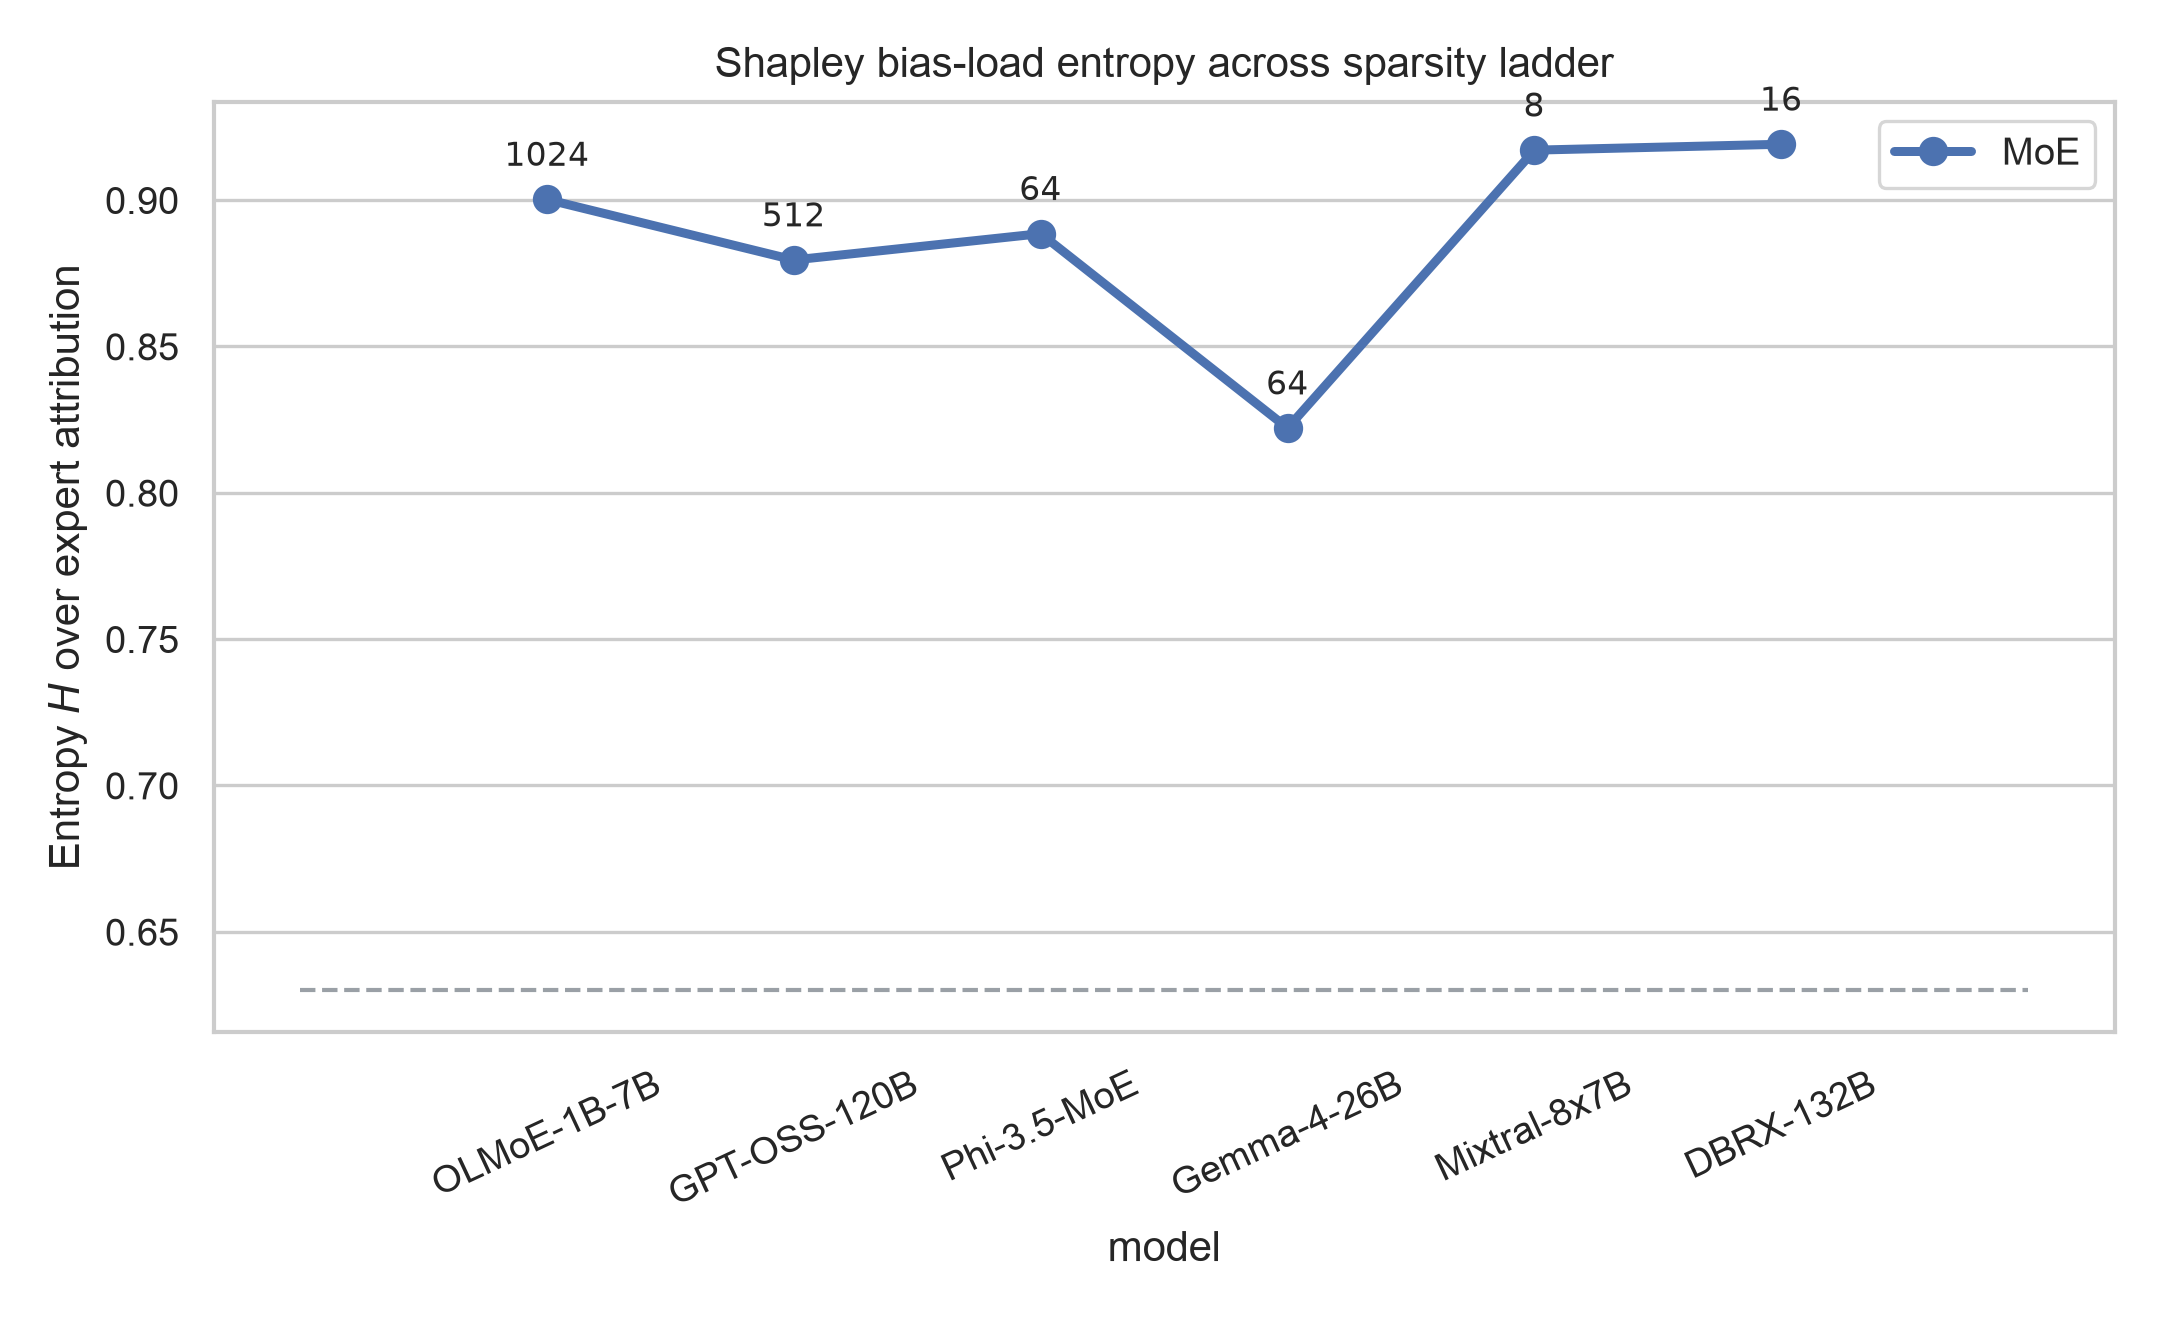
\includegraphics[width=\columnwidth]{fig1_entropy_ladder.png}
\caption{Normalized entropy of the expert attribution across the ladder.
The dashed line is the dense mean.}
\label{fig:ladder}
\end{figure}

\begin{figure}[t]
\centering
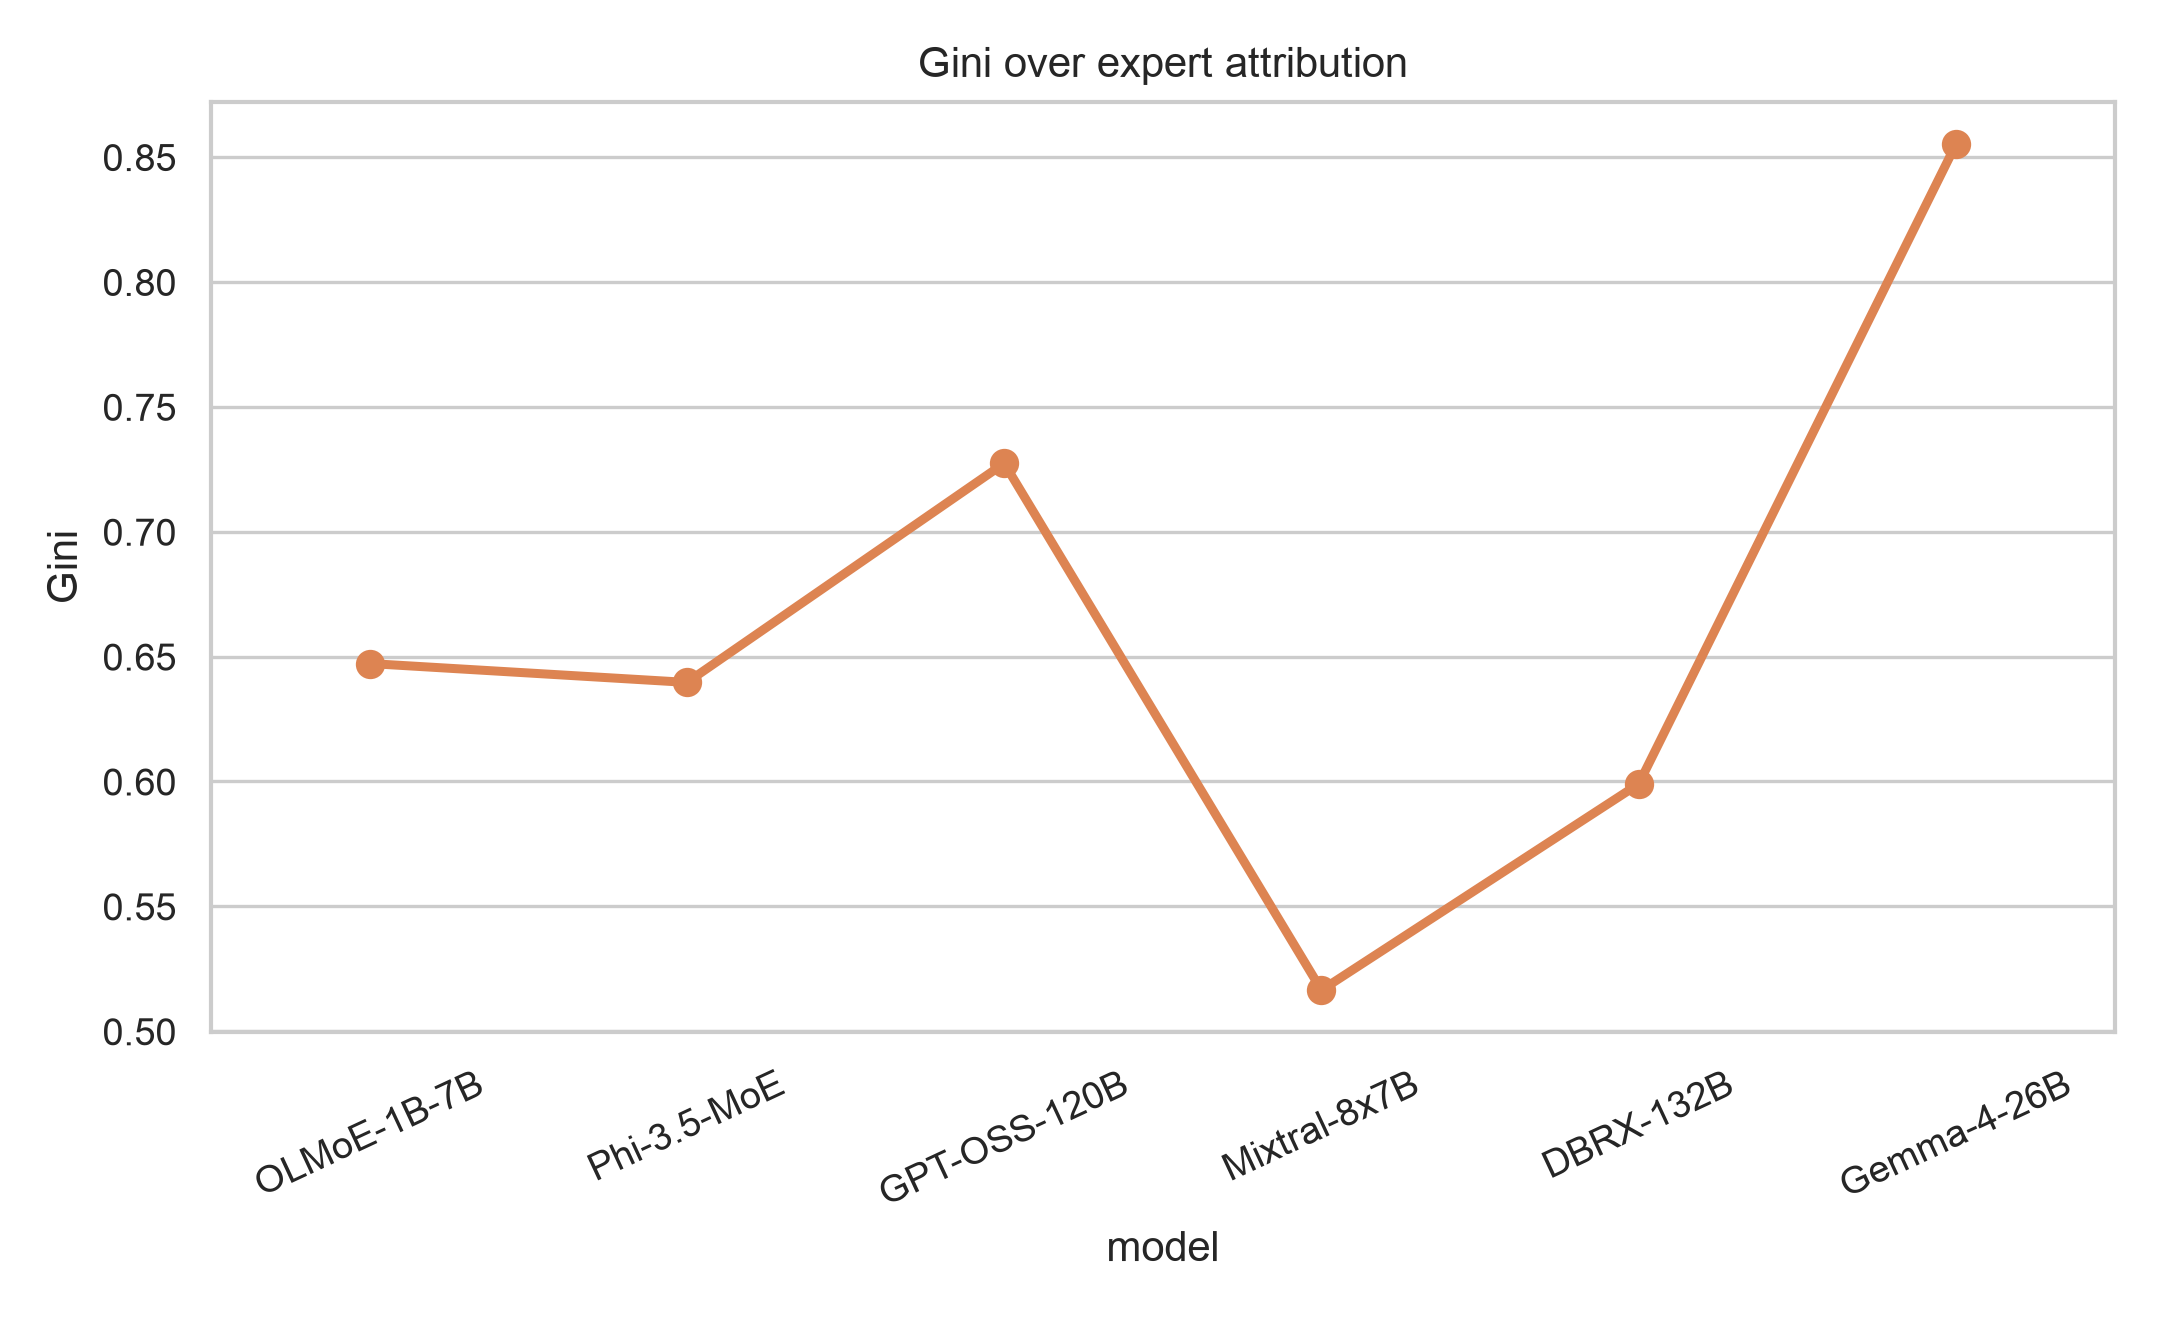
\includegraphics[width=\columnwidth]{fig2_gini_ladder.png}
\caption{Gini of the expert attribution across the ladder.}
\label{fig:gini}
\end{figure}

\begin{figure}[t]
\centering
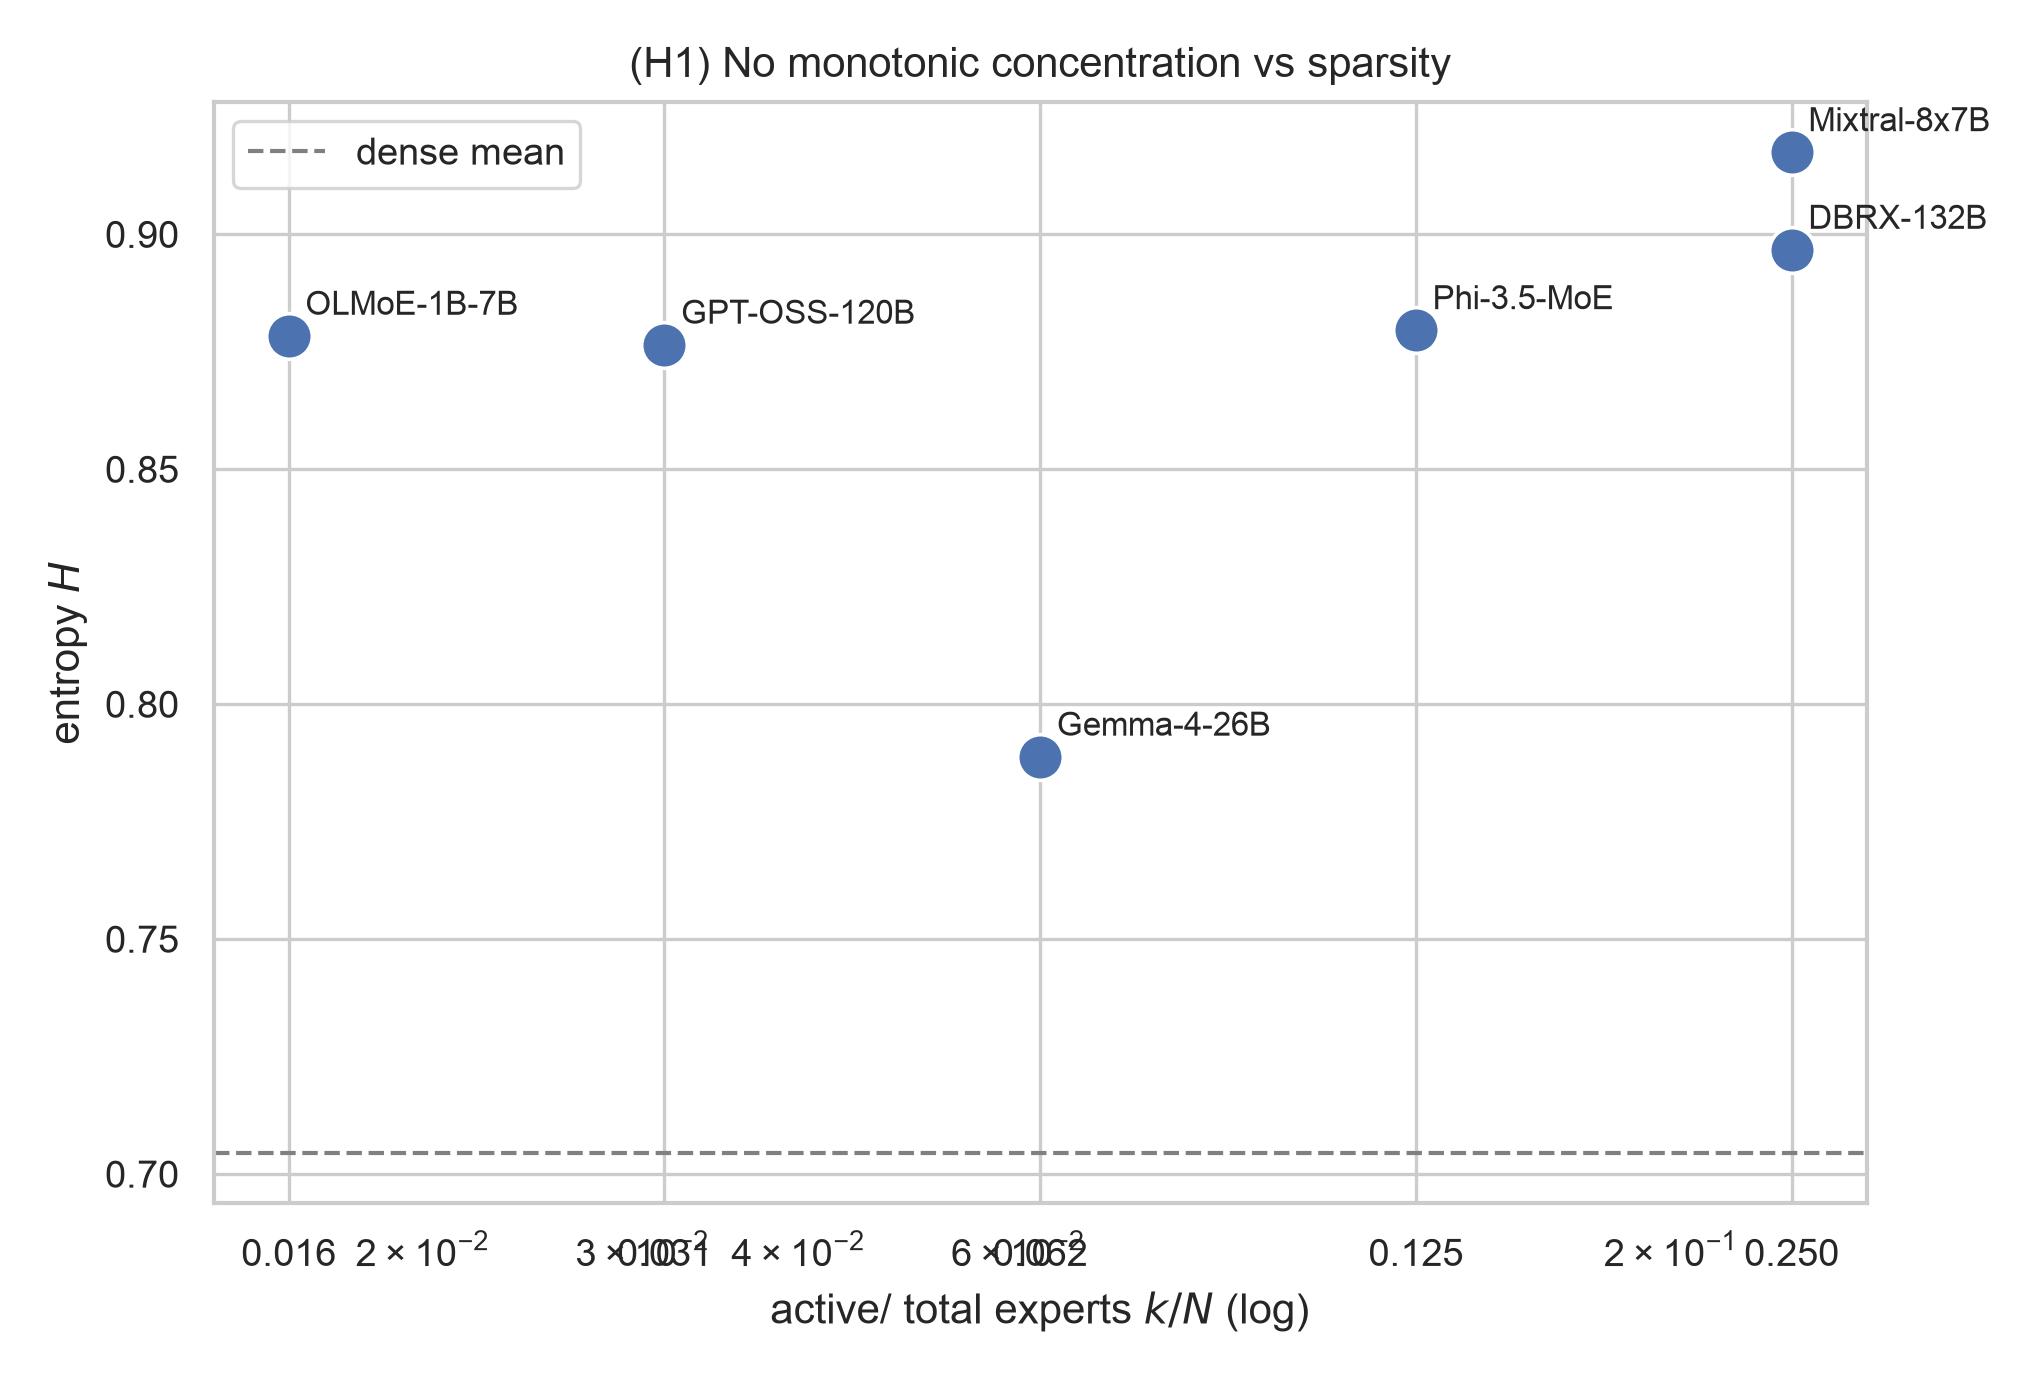
\includegraphics[width=\columnwidth]{fig3_h1_scatter.png}
\caption{Entropy vs.\ active fraction $k/N$ (log scale). H1 (sparser
$\Rightarrow$ more concentrated) is directionally consistent
($\rho_H = +0.754$, exact two-sided permutation $p = 0.106$), but not
statistically significant at $0.05$ given $n = 6$ ladder points.}
\label{fig:scatter}
\end{figure}

\takeaway{Take-away: the sparsity-to-concentration direction holds in the
data, but with six (or fewer) ladder rungs the effect is not statistically
significant---power, not signal, is the limit.}

\subsection{Top-fraction: no expert-level concentration}
Figure~\ref{fig:topfrac}: the top-5 experts hold $2$--$11\%$ of attribution
mass across \emph{all} MoE rungs, and the top-$10\%$ share sits at
$0.35$--$0.77$. There is no small, stable ``fixable'' expert set.

\begin{figure}[t]
\centering
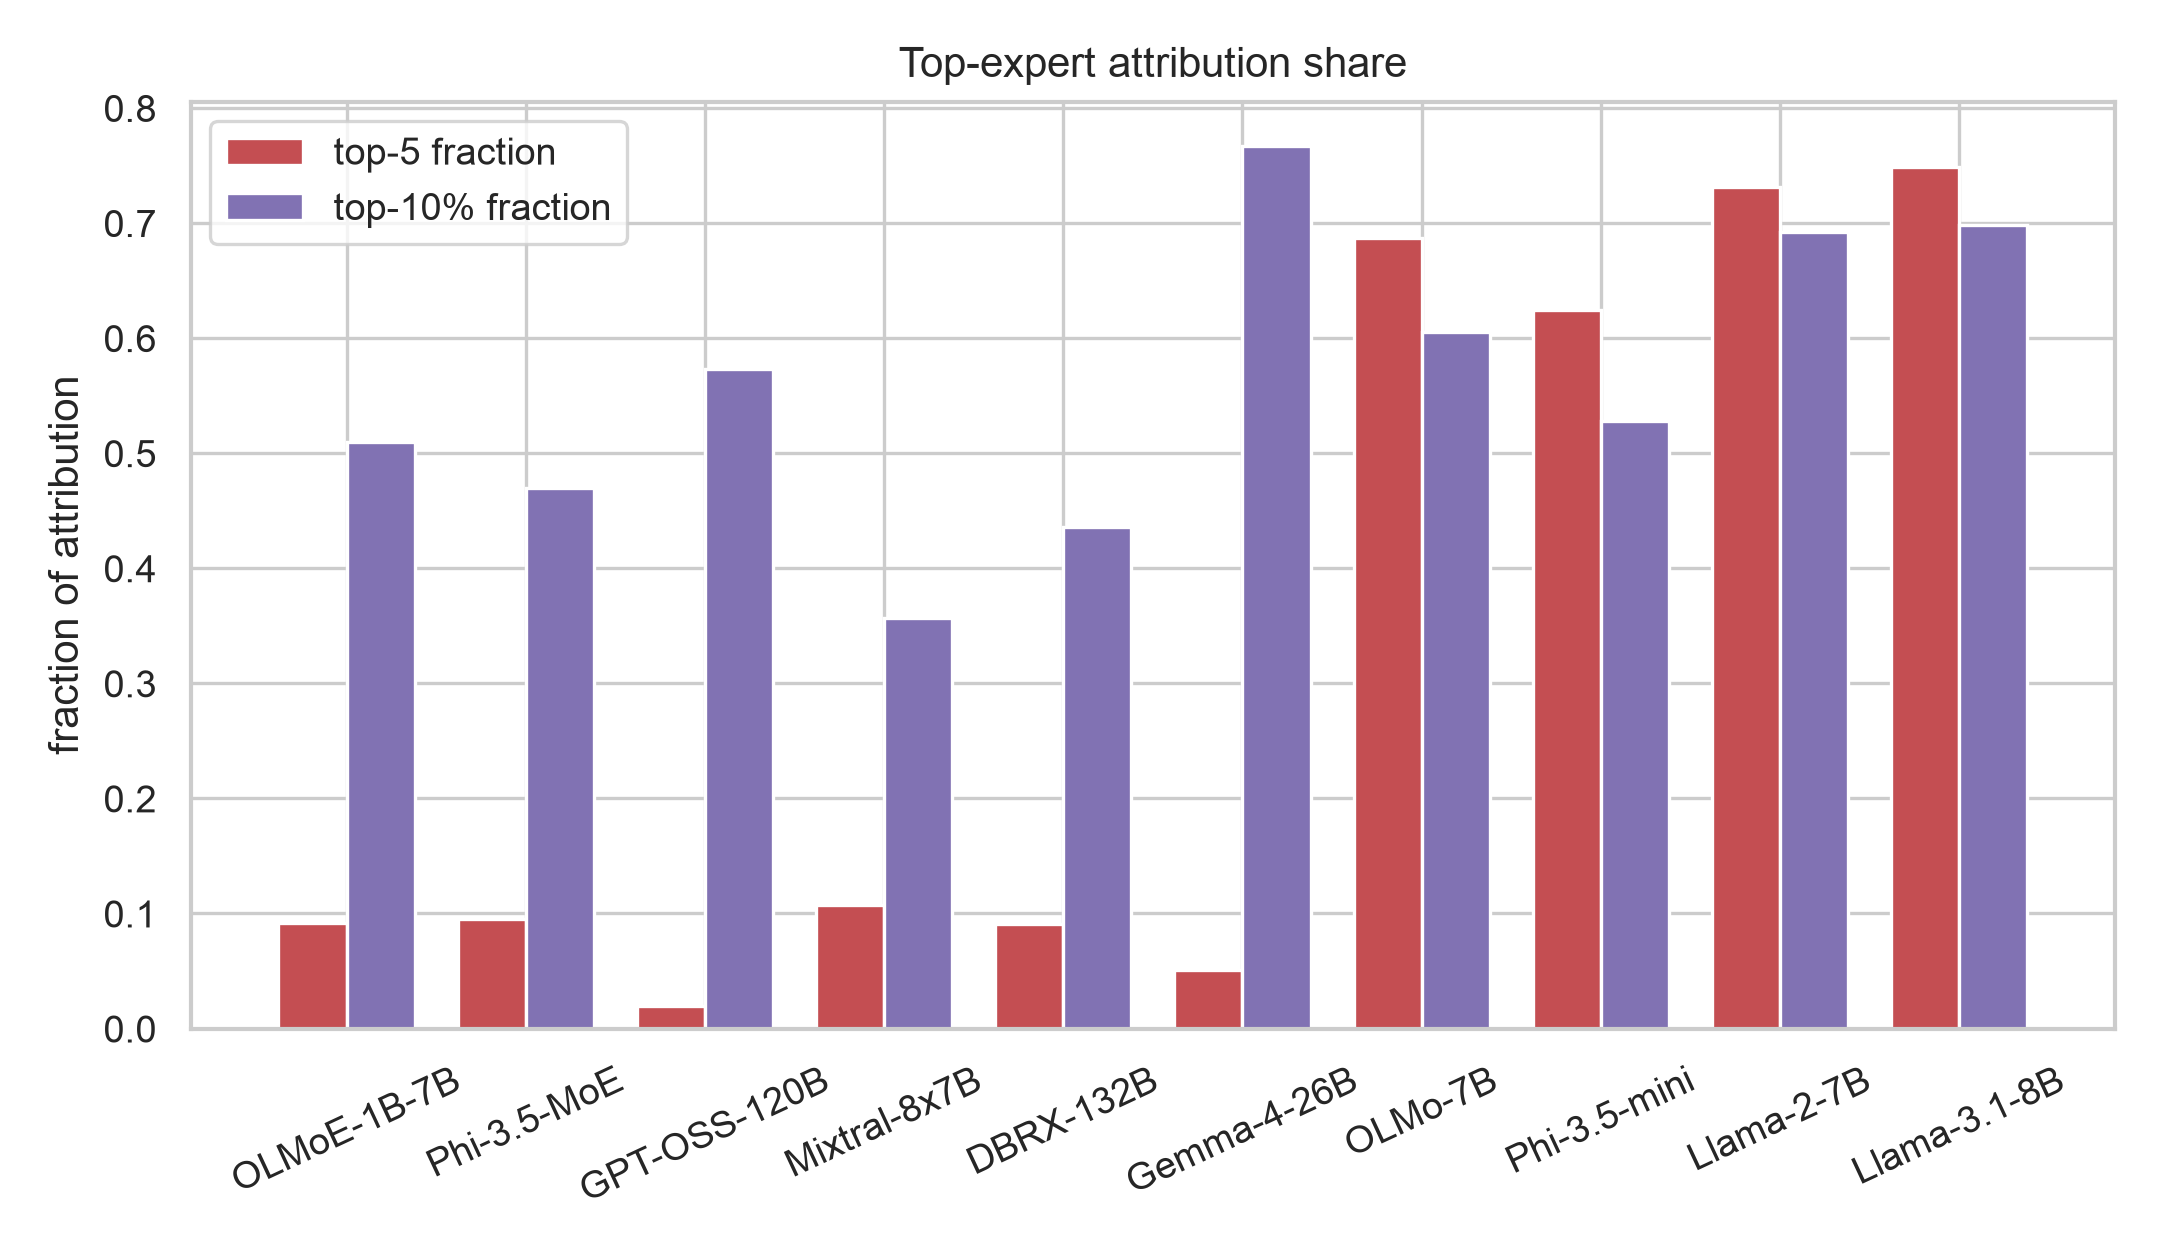
\includegraphics[width=\columnwidth]{fig4_top_fraction.png}
\caption{Top-5 and top-10\% share across the ladder.}
\label{fig:topfrac}
\end{figure}

\subsection{Dense vs.\ MoE: a real split, not a ladder}
Dense baselines ($H$: $0.630$--$0.758$; mean $0.689$, Table~\ref{tab:dense})
cluster clearly below every MoE rung ($0.789$--$0.917$, including the
null-bias Gemma rung). The separation
survives every subset of the ladder and is the robust signal of the
study---but it is a pointer-geometry effect: a dense layer is a single
aggregated player, which mechanically narrows the attribution distribution.
It does not validate bias concentration by the router.

\begin{figure}[t]
\centering
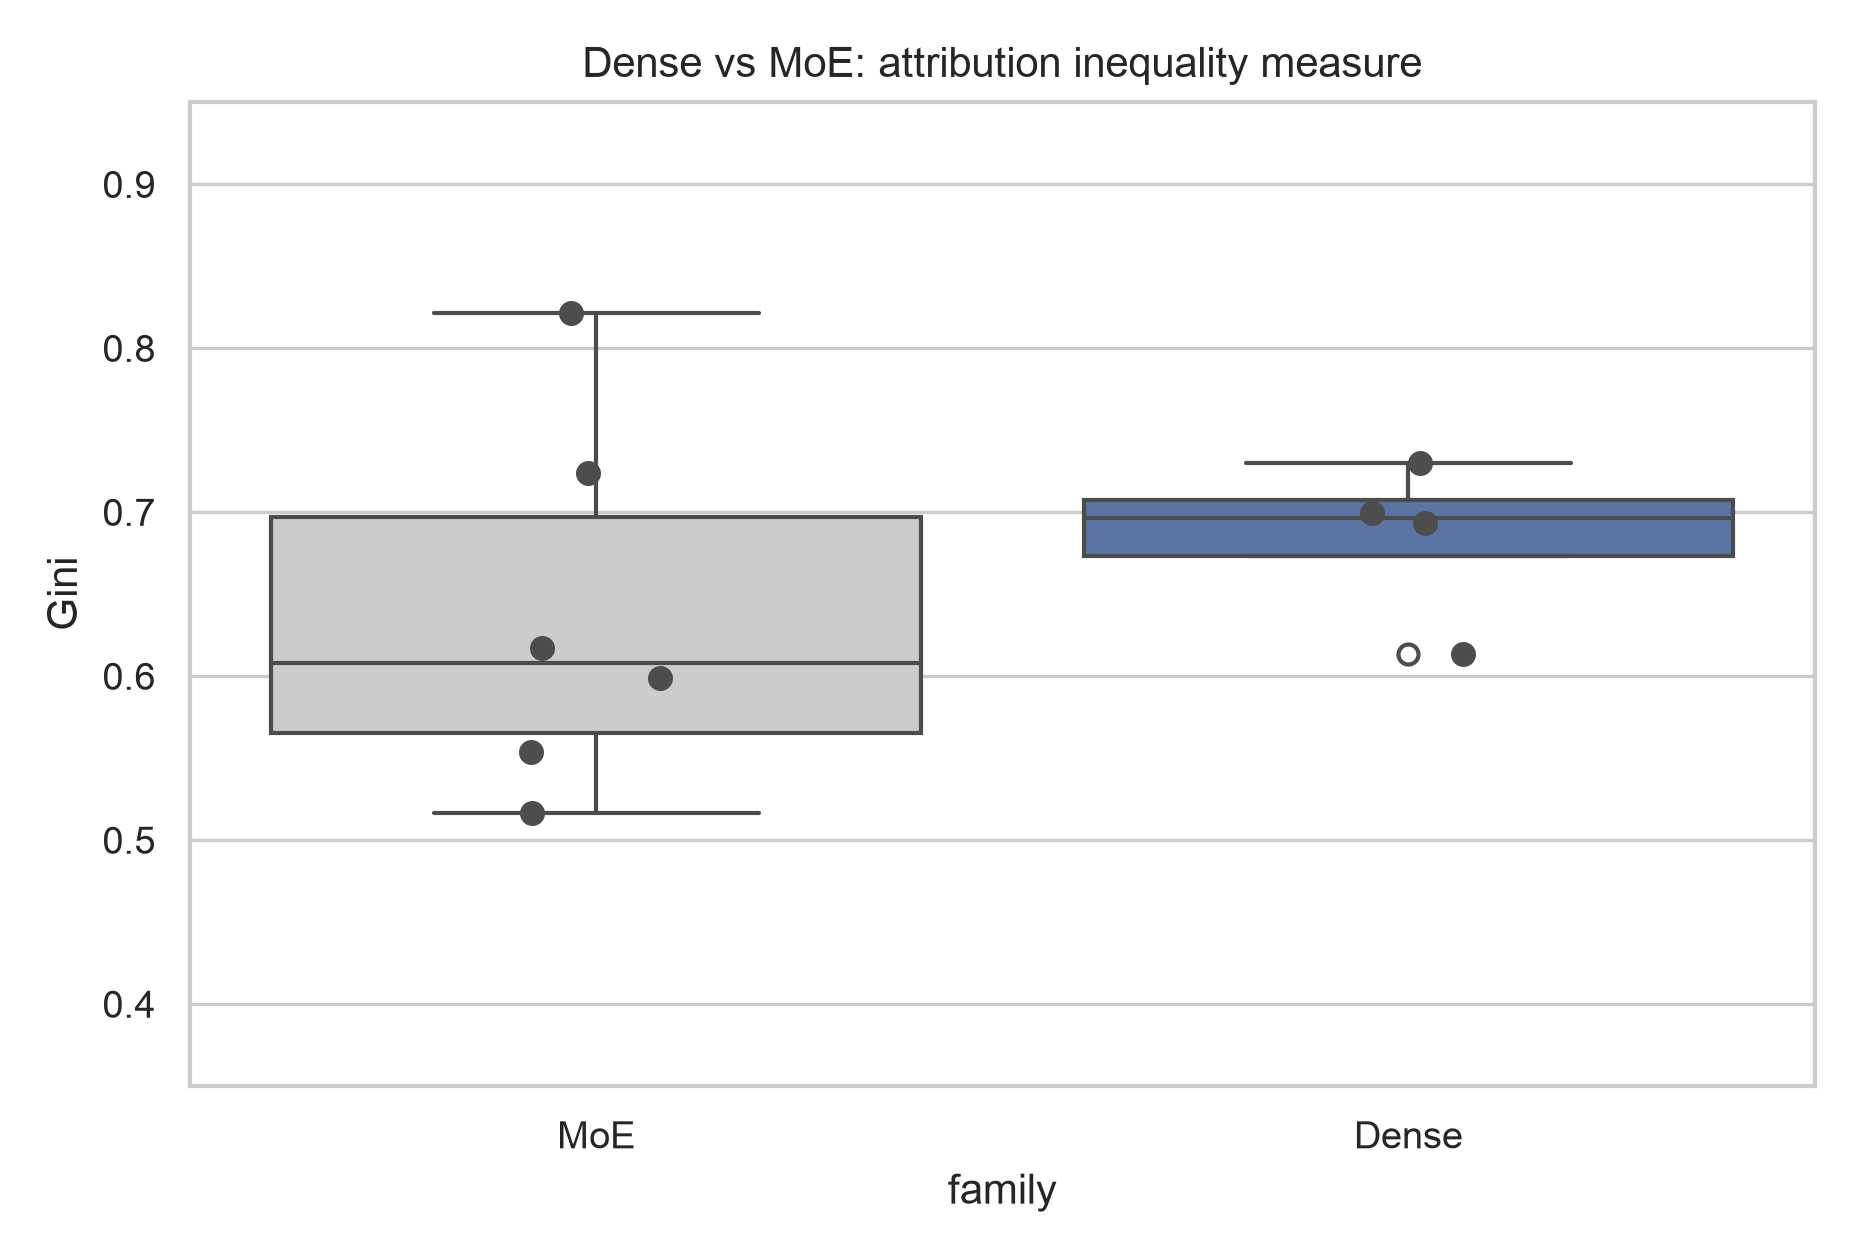
\includegraphics[width=\columnwidth]{fig5_dense_vs_moe.png}
\caption{Dense vs.\ MoE Gini.}
\label{fig:dense}
\end{figure}

\section{Robustness and Sensitivity}
\label{sec:robust}
\subsection{Run-to-run drift (v0 vs.\ v1)}
For the six models captured twice---four MoE models (OLMoE, Phi-3.5-MoE,
Mixtral, DBRX) with 400-pair v0 vs.\ 5000-pair v1 runs, plus GPT-OSS-120B
(400-pair v0 vs.\ valid 2000-pair v1) and Gemma-4-26B (400-pair v0 vs.\
5000-pair v1)---the v0--v1 rerun drift floors are $\mathrm{floor}_H = 0.023$
and $\mathrm{floor}_G = 0.049$ (max absolute drift; mean absolute drift
$0.013$ and $0.024$ respectively). Pairwise ladder differences smaller than
these floors (or than $2\times$ the floor for cross-model comparisons, which
carry error on both sides) are classified as \emph{empirically unresolved};
under that classification the remaining beyond-floor inversions all involve
the null-bias Gemma rung or the GPT-OSS first rung, and no subset's verdict
changes. Split-half shards (two sets of 2500 pairs) for Mixtral/DBRX agree
to $\le 0.004$ in entropy.

\subsection{Permutation / null analysis}
We add (i) an expert-index permutation null that re-shuffles expert
identities within each run, and (ii) a reported-label permutation null
(paper-as-reported; per-prompt assignment not yet shipped, flagged in
Section~\ref{sec:limits}). On the cohort study below, the index null has
mean $0.31$ (sd $0.03$; $p_{95} = 0.37$), and only $0.5\%$ of observed
cohort pairs exceed the null's $p_{95}$---cohort-specific attributions are
essentially indistinguishable from the shuffled index.

\subsection{Model-set sensitivity audit}
\label{sec:verdict}
We re-run the monotonicity verdict across every defensible subset of the
ladder, reporting the exact two-sided permutation $p$-value for $n \le 6$
(all values from \path{outputs/s03_h1_verdict.json}, v1 runs where valid,
v0 otherwise):
\begin{itemize}
\item 6 models (full ladder): $\rho_H = +0.754$, $p = 0.106$; $\rho_G = -0.754$, $p = 0.106$;
\item 5 models (without GPT-OSS): $\rho_H = +0.872$, $p = 0.100$; $\rho_G = -0.872$, $p = 0.100$;
\item 5 models (paper ladder, without Gemma): $\rho_H = +0.872$, $p = 0.100$; $\rho_G = -0.872$, $p = 0.100$;
\item 4 models (without GPT-OSS and Gemma): $\rho_H = +0.949$, $p = 0.167$; $\rho_G = -0.949$, $p = 0.167$;
\item 3 distinct-sparsity rungs: $\rho_H = +1.000$, $p = 0.333$; $\rho_G = -1.000$, $p = 0.333$.
\end{itemize}
Every subset is \emph{SUPPORTED} on point estimates and drift-aware (the
remaining beyond-floor inversions involve only the null-bias Gemma rung and
the GPT-OSS first rung), but no statistic is significant at $p < 0.05$ in
\emph{any} subset: with $n \le 6$ ladder points the attainable
$p$-values are bounded below ($1/12 \approx 0.083$ at $n = 6$, $0.10$ at
$n = 5$, $0.167$ at $n = 4$, $0.333$ at $n = 3$), so the test is
underpowered by construction. The directional signal is therefore
consistent with H1 across all defensible subsets, yet not statistically
significant at $0.05$; power is the limit, not the data.

\subsection{Statistical method note}
All confidence intervals are $95\%$ percentile intervals from a
per-pair block bootstrap: resample the contrastive pairs with replacement,
5000 draws, seed 42, stratified by prompt group for the v1 runs
(\texttt{s04\_bootstrap\_cis.json}). Twelve of thirteen models have per-pair
$\phi$ payloads on disk and are reported in Table~\ref{tab:cis}; only
Gemma-4-27B (not part of the ladder) is MISSING. The cohort JS mean carries
the same bootstrap treatment, $95\%$ CI $[0.206, 0.231]$.

\subsection{Demographic-specificity}
Expanding on OLMoE with 85 demographically-defined cohorts, per-cohort
expert attributions versus the pooled distribution
(\path{exp5-demographic-specificity-olmoe-1b-7b-v1}) show a unimodal
Jensen--Shannon distance distribution with mean $0.22$ (sd $0.05$; bootstrap
$95\%$ CI $[0.206, 0.231]$), far below the expert-index permutation line
$0.31$ (Fig.~\ref{fig:js}); only $0.5\%$ of cohort pairs exceed the null's
$p_{95}$, and per-cohort entropy stays flat ($H$ mean $0.885$, sd $0.026$;
Gini mean $0.638$). No cohort is a ``specialist''---consistent with the
ladder finding. The most divergent pairs (e.g.,
Vietnam$\times$software\_developer, JS $0.27$) do not form a coherent
demographic structure.

\takeaway{Take-away: bias attribution is a routing-structure quantity, not
an expert-level one---no cohort specializes in an expert subset, and no
MoE concentrates bias into a few fixable experts.}

\begin{figure}[t]
\centering
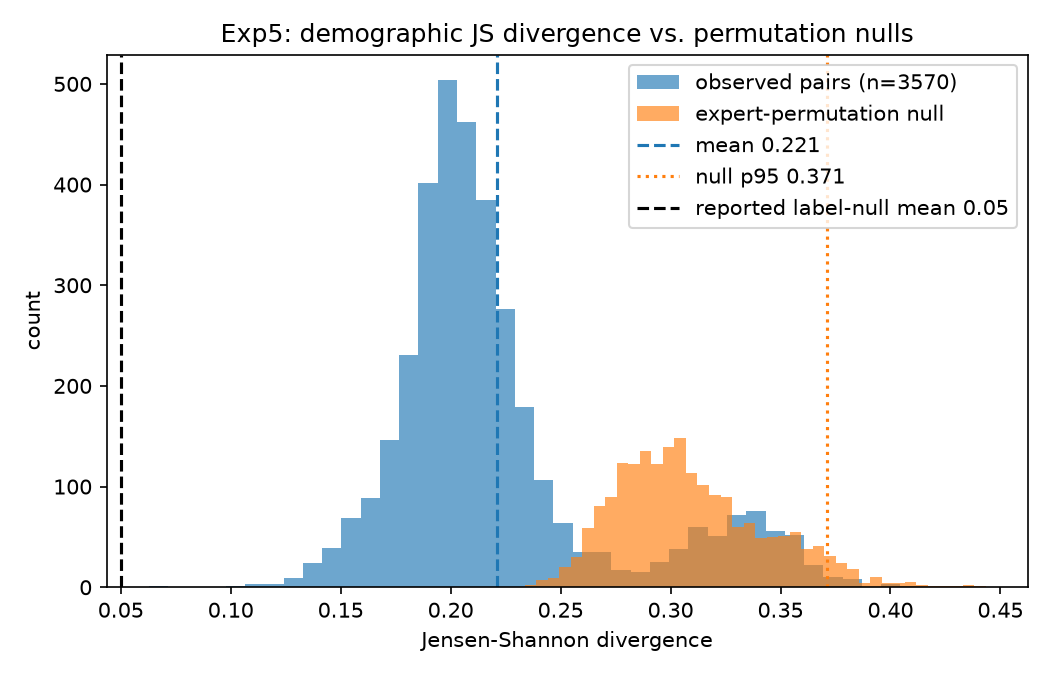
\includegraphics[width=\columnwidth]{s02_js_distribution.png}
\caption{JS distance between per-cohort and pooled expert attribution
distributions (OLMoE, 85 cohorts). The vertical line marks the
expert-index permutation null.}
\label{fig:js}
\end{figure}

\section{Discussion}
The honest picture has two parts. First, the direction: bias attributions
spread broadly across the expert space in every MoE we measured, and the
sparsity-to-concentration trend is monotone-consistent with H1 in every
defensible subset---including the full corrected six-rung ladder after
Gemma's active-expert count was fixed ($N_A$: $960 \rightarrow 240$) and
GPT-OSS-120B's v1 capture was validated. Second, the significance: with
$n \le 6$ ladder points, none of these correlations reaches $p < 0.05$
(all-6 $p = 0.106$; the attainable $p$ is bounded below by $1/12$ on six
points), so the claim ``sparser routing concentrates bias attribution
more'' is directionally supported but statistically unresolved. The single
robust separation is dense-per-layer vs.\ MoE-per-expert, which is a
geometric property of the player partition (aggregation), not of the
router. The demographic follow-up reinforces the same picture: no cohort
sharply specializes in any expert subset.

An apparent tension deserves an explicit resolution. The dense-baseline
comparison and the demographic analysis both ask whether attribution
\emph{geometry}---where mass sits across the routed space---differs
between models or cohorts, and both ``measure'' the same normalized
concentration metrics ($H$, Gini, top fractions) plus Jensen--Shannon
divergence over attribution distributions. None of these quantities
measures the \emph{magnitude} of social bias: a run with zero contrastive
bias (e.g.,\ Gemma-4-26B, whose mean bias gap is $\approx 0$) still yields a
perfectly well-defined routing attribution, and its concentration readings
then describe routing noise. The consistent framing we adopt---for
Exp.~1 entropy \emph{and} Exp.~5 JS divergence alike---is that attribution
geometry is a routing-structure quantity: every concentration or distance
metric inherits the caveat that it characterizes where bias-relevant shift
is localized in the expert/FFN space, not whether or how much bias the
model exhibits. Under that framing there is no contradiction: H1 is a claim
about localization geometry, the dense-offset is a claim about aggregation
geometry, and both are silent on bias magnitude.

Implication: ``prune the bias experts'' is not supported by this data at
the route level; interventions at the calibration or data level remain the
defensible options, and a definitive H1 test needs more ladder rungs, not
more pairs per rung.

\section{Limitations and Uncertainty Flags}
\label{sec:limits}
\begin{itemize}
\item \textbf{GPT-OSS-120B (MXFP4) capture --- resolved.}
Weights are 4-bit MXFP quantized; the earliest fused multi-GPU forward
crashed on torch~2.6 + cu124 (\path{shared_memory_per_block_optin}), and a
first v1 harvest produced an all-zero $\phi$ directory that was discarded.
The current v1 capture is a \emph{valid} 2000-pair run
($H = 0.876$, Gini $0.727$; CI $H$ $[0.875, 0.886]$) used throughout this
paper; it agrees with the v0 bf16-dequantized single-GPU estimate
($\Delta H = -0.003$, $\Delta G = +0.004$).
\item \textbf{Bootstrap CIs --- landed.}
$95\%$ block-bootstrap intervals (5000 resamples over pairs, seed 42,
stratified by prompt group for v1) are reported for every ladder rung in
Table~\ref{tab:cis}; twelve of thirteen model payloads are on disk.
\item \textbf{Gemma-4-26B is a null-bias model --- flag:
\path{null-bias}.} Its mean bias gap $\approx 0$ and $47\%$ of its
$\phi$ are exactly zero; its concentration readings should be treated as
routing noise. Its $k/N$ uses the corrected $N_A = 240$ (an earlier
miscount of $960$ was fixed in \path{s03_h1_verdict.py}). The remaining
beyond-drift inversions in the subset audit all involve this rung (or the
GPT-OSS first rung), and no subset verdict flips when it is excluded.
\item \textbf{Exact permutation $p$ on $n \le 6$ --- flag:
\path{small-n}.} Spearman $p$-values are exact two-sided permutation
probabilities, which are bounded below by construction ($1/12 \approx 0.083$
on 6 points, $0.10$ on 5, $0.167$ on 4, $0.333$ on 3). No subset reaches
$p < 0.05$; we therefore report drift floors, bootstrap intervals, and the
explicit subset audit rather than a binary accept/reject verdict.
\item \textbf{Label-permutation null --- flag: \allowbreak
\path{null:label-pending}.}
The reported-label null in \texttt{s02} was computed as-reported; the
per-prompt assignment is not yet shipped. The expert-index null used here
is on-disk and reproducible.
\item \textbf{Top-$k$ plumbing --- flag: \path{hooks:pending}.} $k$
(active experts) is read from router attributes at runtime
(\path{hooks.py}); DBRX's $N_A$ and any future config divergence may
alter $k/N$ assignment.
\end{itemize}

\section{Conclusion}
Across six MoE models and four dense baselines with a common attribution
kernel, concentration metrics are high and spread out (normalized entropy
$0.789$--$0.917$; top-5 share $2$--$11\%$), with a monotone
sparsity-to-concentration trend that is directionally consistent with H1 in
every defensible subset---all-6 $\rho_H = +0.754$ ($p = 0.106$),
paper-valid-4 $\rho_H = +0.949$ ($p = 0.167$), unique-sparsity-3
$\rho_H = +1.000$ ($p = 0.333$)---but that does not reach statistical
significance at $0.05$ on $n \le 6$ ladder points. The robust signals are
the dense-vs-MoE offset (a player-partition geometry effect) and the
absence of demographic specialist structure. Expert-level pruning of
social bias is not supported as a strategy by this data.

\takeaway{Take-away: the sparsity trend is real in direction and verified on
valid captures, but it is not yet significant---with only six ladder rungs,
power is the limit.}

\section*{Data \& Code}
\begin{itemize}\setlength\itemsep{0pt}
\item Runs and per-pair Shapley payloads:
  \path{expt-bias-1/results/*/result.json}.
\item Analysis scripts: \path{paper_figures_seaborn.py},
  \path{s01_exp1_stability.py}, \path{s02_exp5_js.py},
  \path{s03_h1_verdict.py}, \path{s04_bootstrap_cis.py}
  (all under \path{stats_analysis/scripts/}).
\item Outputs and figures: \path{stats_analysis/outputs/},
  \path{stats_analysis/figures/}.
\end{itemize}

\bibliographystyle{ACM-Reference-Format}
\begin{thebibliography}{99}
\bibitem{shapley1953} L.~S. Shapley. A Value for $n$-Person Games. In
  \emph{Contributions to the Theory of Games II}, Annals of Mathematics
  Studies 28, 1953.
\bibitem{lundberg2017} S.~M. Lundberg and S.-I.~Lee. A Unified Approach to
  Interpreting Model Predictions. In \emph{Advances in Neural Information
  Processing Systems (NeurIPS)}, 2017.
\bibitem{rozemberczki2022} B.~Rozemberczki, L.~Watson, P.~Bayer, H.-T.~Yang,
  O.~Kiss, S.~Nilsson, and R.~Sarkar. The Shapley Value in Machine
  Learning. \texttt{arXiv:2205.10702}, 2022.
\bibitem{shazeer2017} N.~Shazeer, A.~Mirhoseini, K.~Maziarz, A.~Davis,
  Q.~Le, G.~Hinton, and J.~Dean. Outrageously Large Neural Networks: The
  Sparsely-Gated Mixture-of-Experts Layer. In \emph{ICLR}, 2017.
\bibitem{lepikhin2021} D.~Lepikhin, H.~Lee, Y.~Xu, D.~Chen, O.~Firat,
  Y.~Huang, M.~Krikun, N.~Shazeer, and Z.~Chen. GShard: Scaling Giant
  Models with Conditional Computation and Automatic Sharding. In
  \emph{ICLR}, 2021.
\bibitem{fedus2022} W.~Fedus, B.~Zoph, and N.~Shazeer. Switch Transformers:
  Scaling to Trillion Parameter Models with Simple and Efficient Sparsity.
  \emph{Journal of Machine Learning Research}, 23(120):1--39, 2022.
\bibitem{jiang2024} A.~Q.~Jiang \emph{et al.} Mixtral of Experts.
  \texttt{arXiv:2401.04088}, 2024.
\bibitem{muennighoff2024} N.~Muennighoff \emph{et al.} OLMoE: Open
  Mixture-of-Experts Language Models. \texttt{arXiv:2409.12288}, 2024.
\bibitem{gemmaTeam2024} Gemma Team (Google). Gemma: Open Models Based on
  Gemini Research and Technology. \texttt{arXiv:2403.08295}, 2024.
\bibitem{cai2024} Z.~Cai \emph{et al.} A Survey on Mixture of Experts.
  \texttt{arXiv:2407.06204}, 2024.
\bibitem{nadeem2021} M.~Nadeem, A.~Bethke, and S.~Reddy. StereoSet: Measuring
  Stereotypical Bias in Pretrained Language Models. In \emph{ACL}, 2021.
\bibitem{parrish2022} A.~Parrish, A.~Chen, N.~Nangia, V.~Padmakumar,
  J.~Phang, J.~Thompson, P.~M.~Htut, and S.~R.~Bowman. BBQ: A
  Hand-Built Bias Benchmark for Question Answering. In \emph{Findings of
  ACL}, 2022.
\bibitem{liang2023} P.~Liang \emph{et al.} Holistic Evaluation of Language
  Models. \emph{Transactions of the Association for Computational
  Linguistics}, 11:1--48, 2023.
\bibitem{mehrabi2021} N.~Mehrabi, F.~Morstatter, N.~Saxena, K.~Lerman, and
  A.~Galstyan. A Survey on Bias and Fairness in Machine Learning. \emph{ACM
  Computing Surveys}, 54(6):1--35, 2021.
\bibitem{moe_research_2026} MoE-Bias-Research-Group. Routing-Shapley
  Bias-Concentration Study: Code and Artifacts (expt-bias-1), 2026.
\end{thebibliography}

\end{document}
